\subsection{Experimental Setup}

\paragraph{Workloads} Our workloads consist of jobs from public benchmarks -- BigBench (BB) \cite{bbench}, TPC-DS \cite{tpc-ds}, and TPC-H \cite{tpc-h} traces.
A job has multiple phases.
A new phase can be executed if its prerequisite phases are finished.
A phase has a number of equivalent tasks in terms of resource demand and durations.
The cumulative distribution functions (CDFs) task durations across the three benchmarks are presented in Figure \ref{fig:worklad_cdf}.
In each experiment run, we chose the \burstq jobs from one of the traces such that their shortest completion times are less than 30 seconds.
We scale these jobs to make sure their instantaneous demands reach the maximum capacity of a single resource. The \batchq jobs are randomly chosen from one of the traces.
Each \batchq job lasts from tens of seconds to tens of minutes.
Each cluster experiment has 100 \batchq jobs, and each simulation experiment has 500 \batchq jobs.
Throughout the evaluation, all the \batchq jobs are submitted up at the beginning while the \burstq jobs arrive sequentially.
Unless otherwise specified, our default experimental setup has a single \burstq and 8 {\batchq}s.

\begin{figure}[!ht]
	\centering	
	{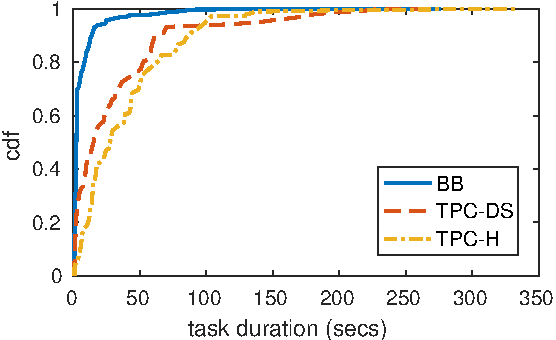
\includegraphics[width=0.8\linewidth]{fig/cdf}}
	\caption{CDFs of task durations across workloads.}
	\label{fig:worklad_cdf}
\end{figure}

\paragraph{User Input} Since the traces give us the resource demand and durations of the job tasks, we can set an ON period equal to the shortest completion time of its corresponding \burstq job.
The average of ON periods is 27 seconds across the traces.
Without loss of generality, we assume that the \burstq jobs arrive periodically
\footnote{The case of aperiodic \burstq jobs is similar to multiple {\burstq}s with different periods.}.
Unless otherwise noted, the inter-arrival period of two \burstq jobs is 300 seconds (1000 seconds) for the cluster experiment (the simulation experiment).

\paragraph{Experimental Cluster}
We setup Apache Hadoop 2.7.2 (YARN) on a cluster having 40 worker nodes on CloudLab~\cite{cloudlab} (40-node cluster).
Each node has 32 CPU cores, 64 GB RAM, a 10 Gbps NIC, and runs Ubuntu 16.04.
Totally, the cluster has 1280 CPU cores and 2.5 TB memory.
The cluster also has a master node with the same specification running the resource manager (RM).

%We emulate the jobs using the Big Bench workload traces. From the traces, we create the jobs that have the same structures, resource demand, and task durations. The jobs are encoded using TEZ and submitted to YARN for scheduling.
%\todo{Not sure what this para says.}

\paragraph{Trace-driven Simulator} To have the experimental results on a larger scale, we build a simulator that mimics the system like Tez atop YARN.
The simulator can replay the directed acyclic graph jobs (like Tez does), and simulate the fair scheduler of YARN at queue level.
For the jobs in the same queue, we allocate the resource to them in a FIFO manner.
Unlike YARN, the simulator supports 6 resources, i.e., CPU, memory, disk in/out throughputs, and network in/out throughputs.

\paragraph{Compared baselines} We compare \name against the following approaches

\begin{enumerate}

\item \textbf{ Dominant Resource Fairness (DRF)}: DRF algorithm is implemented in YARN Fair Scheduler \cite{hadoop-fair-scheduler}.
DRF uses the concept of the dominant resource to compare multi-dimensional resources \cite{drf}.
The idea is that resource allocation should be determined by the dominant share of a queue, which is the maximum share of any resource (memory or CPU). Essentially, DRF seeks to maximize the minimum dominant share across all queues.

\item \textbf{Strict Priority (SP)}: We use Strict Priority to provide the best performance for \burstq jobs.
In fact, we borrow the concept of ``Strict Priority" from network traffic scheduling that enables Strict Priority queues to get bandwidth before other queues \cite{strict_priority}.
Similarly, we enable the {\burstq}s to receive all resources they need first, and then allocate the remaining resources to other queues. If there are conflicts among the {\burstq}s, we use DRF to share the resources among them.

\item \textbf{Naive-BPF (N-BPF)}: N-BPF is a simple version of \name that can provide bounded performance guarantee and fairness.
However, N-\name does not support admission to Soft Guarantee.
For the queues that satisfy the safety condition \ref{eqn:ad-safety}, N-\name decides to admit them to Hard Guarantee if they meet the fairness condition \ref{eqn:ad-fair} and resource condition \ref{eqn:ad-enough}.
Otherwise, it put the queues into the Elastic class. We use N-\name as a baseline when there are multiple {\burstq}s (\S\ref{sec:admission}).

\end{enumerate}
Overall, SP is the upper bound in terms of performance guarantee, and DRF is the upper bound of fairness guarantee for our proposed approach.

\paragraph{Metrics} Our primary metric is the \emph{average completion times} (avg. compl.) of \burstq jobs or \batchq jobs.
To show the performance improvement, we use the average completion times of \burstq jobs across the three approaches.
On the other hand, we use average completion times of \batchq jobs to show that \name also protects the \batchq jobs.
Additionally, we use \emph{factor of improvement} to show how much \name can speed up the \burstq jobs compared to DRF as
$$ \text{Factor of improvement} = \frac{\text{avg. compl. of DRF}}{\text{avg. compl. of \name}}. $$


